% This is the Duke University Statistical Science LaTeX thesis template.
% It has been adapted from the Reed College LaTeX thesis template. The
% adaptation was done by Mine Cetinkaya-Rundel (MCR). Some of the comments
% that are specific to Reed College have been removed.
%
% Most of the work on the original Reed College document class and template
% was done by Sam Noble (SN). Later comments etc. by Ben Salzberg (BTS).
% Additional restructuring and APA support by Jess Youngberg (JY).
%
% See https://www.reed.edu/cis/help/latex/ for help. There are a
% great bunch of help pages there, with notes on
% getting started, bibtex, etc. Go there and read it if you're not
% already familiar with LaTeX.
%
% Any line that starts with a percent symbol is a comment.
% They won't show up in the document, and are useful for notes
% to yourself and explaining commands.
% Commenting also removes a line from the document;
% very handy for troubleshooting problems. -BTS

%%
%% Preamble
%%
% \documentclass{<something>} must begin each LaTeX document
\documentclass[12pt,oneside]{dukestatscithesis}
% Packages are extensions to the basic LaTeX functions. Whatever you
% want to typeset, there is probably a package out there for it.
% Chemistry (chemtex), screenplays, you name it.
% Check out CTAN to see: http://www.ctan.org/
%%
\usepackage{graphicx,latexsym}
\usepackage{amsmath}
\usepackage{amssymb,amsthm}
\usepackage{longtable,booktabs,setspace}
\usepackage{chemarr} %% Useful for one reaction arrow, useless if you're not a chem major
\usepackage[hyphens]{url}
% Added by CII
\usepackage{hyperref}
\usepackage{lmodern}
\usepackage{float}
\floatplacement{figure}{H}
% End of CII addition
\usepackage{rotating}

% Next line commented out by CII
%%% \usepackage{natbib}
% Comment out the natbib line above and uncomment the following two lines to use the new
% biblatex-chicago style, for Chicago A. Also make some changes at the end where the
% bibliography is included.
%\usepackage{biblatex-chicago}
%\bibliography{thesis}


% Added by CII (Thanks, Hadley!)
% Use ref for internal links
\renewcommand{\hyperref}[2][???]{\autoref{#1}}
\def\chapterautorefname{Chapter}
\def\sectionautorefname{Section}
\def\subsectionautorefname{Subsection}
% End of CII addition

% Added by CII
\usepackage{caption}
\captionsetup{width=5in}
% End of CII addition

% \usepackage{times} % other fonts are available like times, bookman, charter, palatino


% To pass between YAML and LaTeX the dollar signs are added by CII
\title{EAS 499 Final Thesis}
\author{Ali Kozlu}
% The month and year that you submit your FINAL draft TO THE LIBRARY (May or December)
\date{Dec 2018}
\advisor{Professor Marcus Mitchell}
\institution{University Of Pennsylvania}
\degree{Bachelor of Science in Computer and Cognitive Science}
%\committeememberone{}
%\committeemembertwo{}
%\dus{}
%If you have two advisors for some reason, you can use the following
% Uncommented out by CII
% End of CII addition

%%% Remember to use the correct department!
\department{Department of Computer and Cognitive Science}

% Added by CII
%%% Copied from knitr
%% maxwidth is the original width if it's less than linewidth
%% otherwise use linewidth (to make sure the graphics do not exceed the margin)
\makeatletter
\def\maxwidth{ %
  \ifdim\Gin@nat@width>\linewidth
    \linewidth
  \else
    \Gin@nat@width
  \fi
}
\makeatother

\renewcommand{\contentsname}{Table of Contents}
% End of CII addition

\setlength{\parskip}{0pt}

% Added by CII
  %\setlength{\parskip}{\baselineskip}
  \usepackage[parfill]{parskip}

\providecommand{\tightlist}{%
  \setlength{\itemsep}{0pt}\setlength{\parskip}{0pt}}

\Acknowledgements{

}

\Dedication{

}

\Preface{

}

\Abstract{
The NFL player tracking data presents an unique opportunity to
automatize the process of breaking down film and tagging routes. More
importantly, it gives an opportunity to examine methods to classify
pattern of routes, so called route concepts. The present research will
attempt to identify an already chosen route concept, using a combination
of features devised from receiver route trajectories and certain
characteristics regarding the specified route concept in pass plays. The
hope is that this work will be complementary to an unsupervised machine
learning model of basic route identification, which will be addressed in
an upcoming paper. The eventual goal is to use a route identification
model with a framework of identfying concepts in order to streamline the
process of finding plays accross the NFL that include the same pass
concept.
}

	\usepackage{amsmath}
	\usepackage{float}
	\usepackage{booktabs}
	\usepackage{longtable}
	\usepackage{array}
	\usepackage{multirow}
	\usepackage[table]{xcolor}
	\usepackage{wrapfig}
	\usepackage{float}
	\usepackage{colortbl}
	\usepackage{pdflscape}
	\usepackage{tabu}
	\usepackage{threeparttable}
	\usepackage{threeparttablex}
	\usepackage[normalem]{ulem}
	\usepackage{makecell}
	\usepackage{xcolor}
% End of CII addition
%%
%% End Preamble
%%
%

\usepackage{amsthm}
\newtheorem{theorem}{Theorem}[chapter]
\newtheorem{lemma}{Lemma}[chapter]
\theoremstyle{definition}
\newtheorem{definition}{Definition}[chapter]
\newtheorem{corollary}{Corollary}[chapter]
\newtheorem{proposition}{Proposition}[chapter]
\theoremstyle{definition}
\newtheorem{example}{Example}[chapter]
\theoremstyle{definition}
\newtheorem{exercise}{Exercise}[chapter]
\theoremstyle{remark}
\newtheorem*{remark}{Remark}
\newtheorem*{solution}{Solution}
\begin{document}

% Everything below added by CII
  \maketitle

\frontmatter % this stuff will be roman-numbered
\pagestyle{empty} % this removes page numbers from the frontmatter



  \hypersetup{linkcolor=black}
  \setcounter{tocdepth}{2}
  \tableofcontents

  \listoftables

  \listoffigures
  \begin{abstract}
    The NFL player tracking data presents an unique opportunity to
    automatize the process of breaking down film and tagging routes. More
    importantly, it gives an opportunity to examine methods to classify
    pattern of routes, so called route concepts. The present research will
    attempt to identify an already chosen route concept, using a combination
    of features devised from receiver route trajectories and certain
    characteristics regarding the specified route concept in pass plays. The
    hope is that this work will be complementary to an unsupervised machine
    learning model of basic route identification, which will be addressed in
    an upcoming paper. The eventual goal is to use a route identification
    model with a framework of identfying concepts in order to streamline the
    process of finding plays accross the NFL that include the same pass
    concept.
  \end{abstract}

\mainmatter % here the regular arabic numbering starts
\pagestyle{fancyplain} % turns page numbering back on

Bounce rate defined as: the percentage of visitors to a particular
website who navigate away from the site after viewing only one page. \#
Introduction \{.unnumbered\} This report was commissioned to investigate
the results our recent A/B test. The goal was to test a potential change
to the categories displayed on our mobile home page. The suggested
adjustment was to display the 10 categories nearest to the user's
location, instead of displaying the 10 most popular categories based on
sales. Much of our analysis will use two main metrics, namely conversion
and bounce rate, to see how much revenue and click rate is earned in
each variation. The relevant data gathered for each user profile can be
seen in \ref{tab:datasetbreakdown}. the NFL teams spend a significant
amount of time each week breaking down film and tagging play in search
of opponent tendencies and patterns. In addition, the staff pays
attention to what other offenses around the league are doing to compare
the revenue and click rate generation of two variations. and if they can
``steal'' plays from other teams to add to their playbook. A coach can,
for example, look what concepts the other teams are running from a
particular formation and adapt a certain version of that play to their
playbook. This process is very time intensive, as it requires the staff
to go through all the film and label (tagging) play data by hand. It is
almost certain that with the NFL's available player tracking data, this
process will soon be automatized through unsupersived machine learning
models. However, even if the routes are labeled according to models, a
route is only a vector (meaning that it has a specific direction and
speed) movement taken by a specific receiver. A better input to the
staff is to classify is a pre-packaged pattern of routes, which is
usually denoted as a route concept. Thus the aim of the route classifier
is to use the information as input to identify a route concept, as done
in real life film tagging. Which concepts to classify is dependent to
input from the staff, as we can try to classify medium pass level
concepts such as levels or mesh concepts. We can also choose to classify
higher level concepts such as rub route plays, which can come from
different formations and different route combinations. The goal of the
present thesis is to see how a singular concept can be classified using
trajectory data. Specifically it attempts to use state of the art
patiotemporal information systems from fields such as biology and
GPS-tracking to classify routes into a stem, pivot (turning point) and
branch components and identify a rub route concept, the slant-flat. In
doing so, it will explore appropriate means of feature engineering for
route evaluation, and specific challenges of classifying route concepts.
\^{}{[}You can find the Python script used for this project
\href{https://github.com/akozlu/NFLModel}{here.}
\begin{longtable}[]{@{}lc@{}}
\caption{\label{tab:datasetbreakdown} Breakdown of the dataset used for
experiment}\tabularnewline
\toprule
\begin{minipage}[b]{0.60\columnwidth}\raggedright\strut
Column Explanation\strut
\end{minipage} & \begin{minipage}[b]{0.24\columnwidth}\centering\strut
Data Columns\strut
\end{minipage}\tabularnewline
\midrule
\endfirsthead
\toprule
\begin{minipage}[b]{0.60\columnwidth}\raggedright\strut
Column Explanation\strut
\end{minipage} & \begin{minipage}[b]{0.24\columnwidth}\centering\strut
Data Columns\strut
\end{minipage}\tabularnewline
\midrule
\endhead
\begin{minipage}[t]{0.60\columnwidth}\raggedright\strut
Date of user's visit\strut
\end{minipage} & \begin{minipage}[t]{0.24\columnwidth}\centering\strut
Date\strut
\end{minipage}\tabularnewline
\begin{minipage}[t]{0.60\columnwidth}\raggedright\strut
How the user arrived at our website\strut
\end{minipage} & \begin{minipage}[t]{0.24\columnwidth}\centering\strut
Channel\strut
\end{minipage}\tabularnewline
\begin{minipage}[t]{0.60\columnwidth}\raggedright\strut
New or returning visitor to the website\strut
\end{minipage} & \begin{minipage}[t]{0.24\columnwidth}\centering\strut
User Type\strut
\end{minipage}\tabularnewline
\begin{minipage}[t]{0.60\columnwidth}\raggedright\strut
1 if landed directly, 0 if navigated from another page on our site\strut
\end{minipage} & \begin{minipage}[t]{0.24\columnwidth}\centering\strut
Land\strut
\end{minipage}\tabularnewline
\begin{minipage}[t]{0.60\columnwidth}\raggedright\strut
1 if left website after landing, 0 if navigated to another page after
landing\strut
\end{minipage} & \begin{minipage}[t]{0.24\columnwidth}\centering\strut
Bounce\strut
\end{minipage}\tabularnewline
\begin{minipage}[t]{0.60\columnwidth}\raggedright\strut
1 if purchased, else 0\strut
\end{minipage} & \begin{minipage}[t]{0.24\columnwidth}\centering\strut
Purchase\strut
\end{minipage}\tabularnewline
\begin{minipage}[t]{0.60\columnwidth}\raggedright\strut
Number of visitors in control that satisfy above criterion\strut
\end{minipage} & \begin{minipage}[t]{0.24\columnwidth}\centering\strut
Visitors\_Variant\strut
\end{minipage}\tabularnewline
\begin{minipage}[t]{0.60\columnwidth}\raggedright\strut
Number of visitors in control that satisfy above criterion\strut
\end{minipage} & \begin{minipage}[t]{0.24\columnwidth}\centering\strut
Visitors\_Control\strut
\end{minipage}\tabularnewline
\bottomrule
\end{longtable}
\chapter{A/B Test Analysis}\label{rmd-basics}

\section{Comparison of Key Metrics}\label{comparison-of-key-metrics}

Previous attempts to identify American Football Routes and formations
were done by using computer vision techniques looking at pixel density
and weighted spatial of All-22 film. Ajmeri \& Sha (2018) use this data
to extract features such as quarterback position, number, and location
of tight ends, running backs and receivers to identify formations.
Jeremy \& Gagnon (2017) utilize radio-frequency identification (RFID)
tracking technology to monitor post-snap on field locations of offensive
players. The 231 routes they extracted were then classified manually and
then trained by a Naive-Bayes model. The most innovative aspect about
work of Jeremy \& Gagnon (2017) is how they apply their knowledge of the
football domain to generate important feature extraction metrics from
receiver routes. As they explain, basic receiver routes are comprised of
three essential components: a stem, pivot, and branch. In order to
extract important features such as stem length and branch direction, one
has to first establish the turning points of receivers from trajectory
data. They use Segmented Euclidean Regression, where they go over each
frame and test each point in the route as a possible pivot point. The
point with minimal Euclidean Error is established as route's true pivot
point. Although mathematically sound, one can argue that this approach
is far from perfect empirically. Although a good approximation, it takes
\(O(n^{2})\) time where n denotes the number of frames, making it highly
slow in practice. We start by exploring an alternative method that can
find ``valuable'' turning points by constructing an approximated
trajectory. It should also be mentioned that frame by frame direction
data provided by the dataset can be deceiving when trying to establish
turning points, as the direction change takes multiple frames to
complete, making it hard to use direction data to pinpoint the turning
point the players.
\begin{figure}
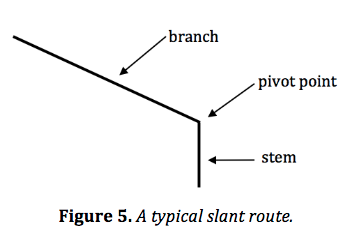
\includegraphics[width=4.88in,angle=360, scale=1]{figure/routes} \caption{Figure taken}\label{fig:routepicture}
\end{figure}
\section{Ramer-Douglas-Peucker
algorithm}\label{ramer-douglas-peucker-algorithm}

Basicly put, Ramer-Douglas-Peucker algorithm, based on papers of
Beckmann \& Budig (2015), H \& Peucker (1973) and Urs. (1973), is an
algorithm for reducing the number of points in a curve that is
approximated by a series of points. The implementation of the algorithm
in O(n logn) time in Python can be found
\href{https://github.com/fhirschmann/rdp}{here.} It does so by creating
a simplified trajectory and finding turning turnings in between piece
wise segments. The two figures below demonstrate the start and finish
trajectories of the algorithm. The black points in the second figure
represent the turning points found by using segmenting initial
trajectories into simple trajectories.
\begin{figure}
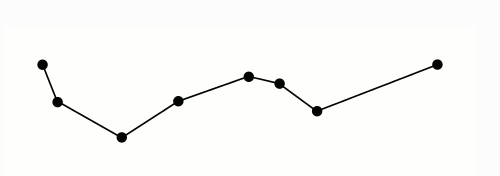
\includegraphics[width=6.94in,angle=360, scale=0.5]{figure/rdp1} \caption{Initial trajectory}\label{fig:rdp}
\end{figure}
\begin{figure}
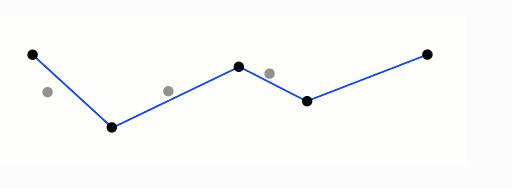
\includegraphics[width=7.11in,angle=360, scale=0.5]{figure/rdp2} \caption{Turning points of simplified trajectory}\label{fig:rdp2}
\end{figure}
\section{Application of RDP Algorithm to Play
Data}\label{application-of-rdp-algorithm-to-play-data}

We can apply the above-described algorithm to find turning points in
routes run by receivers in passing plays. Below is the simplified
trajectory data from the same example play on NFL Football Operations
Github Page, the 75-yard Tyreek Hill Touchdown from the Week 1 game
between New England Patriots and Kansas City Chiefs. For simplification,
only the trajectories of Chiefs receivers are displayed. In the graph,
the starting ball point (the black circle) represents the origin (0,0).
Every other player starting position at ball snap it adjusted
accordingly.\footnote{This method will also be used in future to train a
  route classifier. The starting position of the receiver in respect to
  the ball from both sides can a valuable feature for successfully
  classifying routes.} In this play, we see 2 stacked receivers on each
side of the ball. The routes of players are simplified using the
Ramer-Douglas-Peucker algorithm. The red dots represent the valuable
turning points in these simplified trajectories. The black cross
presents the point where the pass was thrown.
\begin{figure}
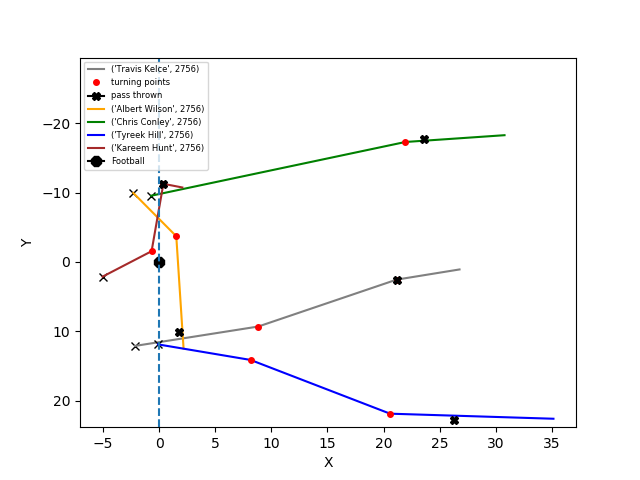
\includegraphics[width=8.89in,angle=360, scale=0.6]{figure/2756_simple} \caption{A.Smith pass deep right to T.Hill for 75 yards. Light blue dashed line is the line of scrimmage. Ball on the right hashmark. Simplified trajectories are shown}\label{fig:2756simple}
\end{figure}
We can then extract these turning points and save their location
alongside the initial trajectories. Below is the same play, but the red
turning points are displayed on initial trajectories. After extracting
stem length, turning point and branch of every route, we can use this
information to identify a certain concept in a play. Before doing so,
additional information may be required in order to identify the concept,
which is explained through an example in the next chapter.
\begin{figure}
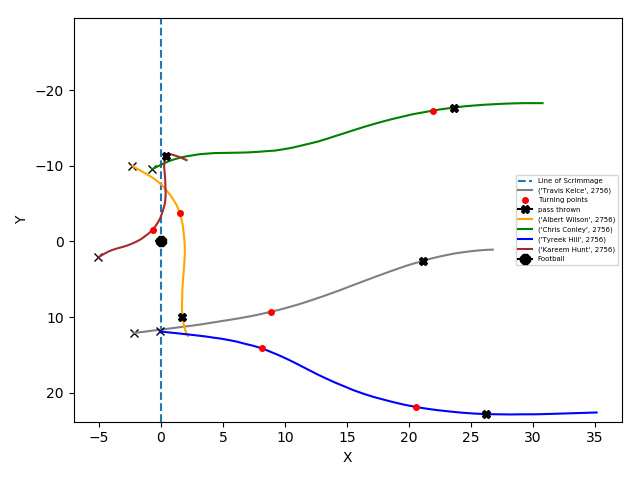
\includegraphics[width=8.89in,angle=360, scale=0.6]{figure/2756} \caption{The original trajectories of receivers alongside their turning points.}\label{fig:2756complex}
\end{figure}
\chapter{Identying A Certain Route Concept}\label{math}

\section{The Rub Concept}\label{the-rub-concept}

Simply put, the Rub Concept designs two or more receivers routes in the
same area so that receivers can run their defenders into
combined-traffic, creating seperation for one or both receivers. A
version of rub concept occurs when two receivers on the same side run a
flat-slant combination. This concept can be run from multiple offensive
looks, such as Trips, Dubs formations or empty sets, as shown in the
pictures below.
\begin{figure}
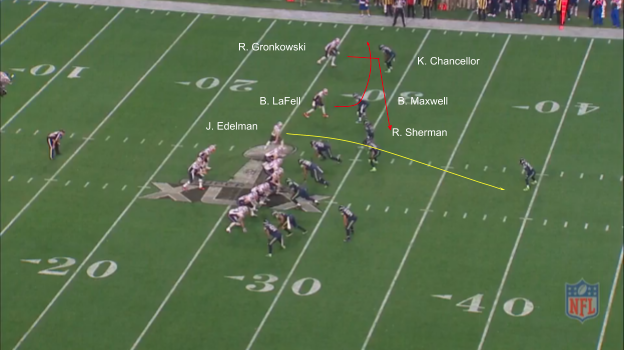
\includegraphics[width=8.72in,angle=360, scale=0.5]{figure/rub2} \caption{ Slant-Flat Rub Concept from different looks}\label{fig:rubimages}
\end{figure}\begin{figure}
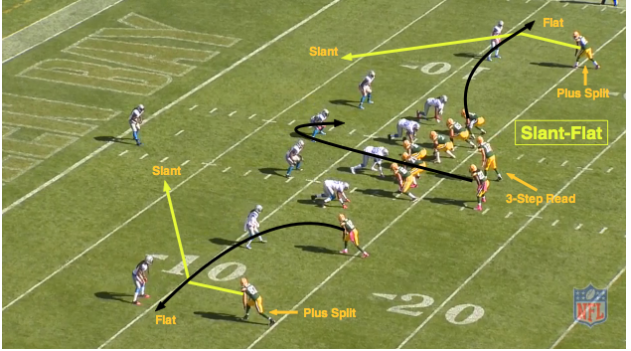
\includegraphics[width=8.76in,angle=360, scale=0.5]{figure/rub4} \caption{ Slant-Flat Rub Concept from different looks}\label{fig:rubimages}
\end{figure}
In order to identify a slant flat rub route concept, we must
automatically detect certain additional features from receiver
trajectories. Firstly, we can check whether two receiver trajectories
intersect at a given point, which is essential to create traffic in a
certain area of the field. This is not enough however, since we can
observe trajectory intersections in other concepts such as the mesh
concept as well. Thus we have to limit the pair of trajectories we
investigate between players who are on the same side of the formation
(i.e.~same side of the ball). Moreover, in the slant-flat concept, the
intersection occurs (most of the time) within 5 yards of line of
scrimmage. The script written for this project achieves this by grouping
the receivers to left and right hand side of the ball and checking if
combination of routes for two receivers on the sime side intersect
within 5 yards of line of scrimmage. Since the trajectories we observe
we observe these three criterion in a play, alongside with turning
points associated with slant and flat routes, we add the play to our
database and display it.

\section{Determining Route
Intersection}\label{determining-route-intersection}

Since the trajectories of players cannot be defined by lines, they
cannot be defined by simple parametrized functions. Thus in order to do
a deterministic spatial analysis of intersection, we treat the routes as
Polygons and use the
\href{https://shapely.readthedocs.io/en/latest/manual.html\#introduction}{Shapely
library}, which is a Python package for set-theoretic analysis and
manipulation of planar features using. Given two polygons, the library
can determine whether the two intersect at any given point, as the
spatial data model provided by the library is able to evualute
\emph{intersects} relationship between two polygons.

\section{Identfying Slant-Flat
Concept}\label{identfying-slant-flat-concept}

As mentioned above if two receivers in a play have turning points, stem
length and branches associated with slant and flat routes and their
routes intersect within 5 yards of line of scrimmage on a certain side
of the ball, we flag the play and add it to a certain database. Running
the script on the Chiefs vs.~Patriots game, we flag the play below as a
slant-flat concept on the right hand side of the field as it succesfully
satisfies each of our criteria.
\begin{figure}
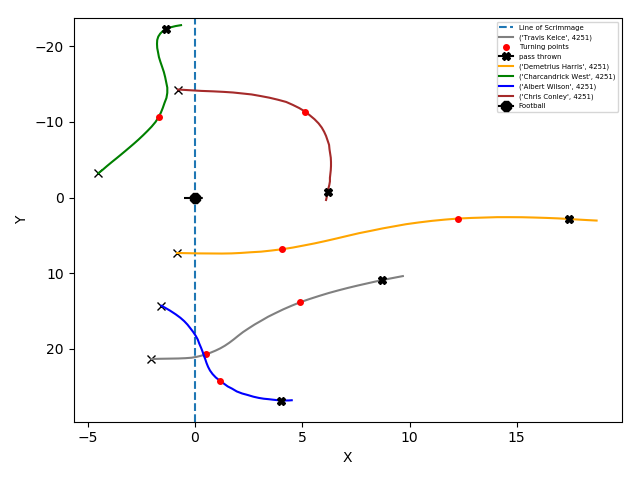
\includegraphics[width=8.89in,angle=360, scale=0.6]{figure/4251} \caption{Ball on left hashmark. On the right hand side, Kelce runs a slant and Wilson goes to the flat. Play is added to database }\label{fig:slantflat1}
\end{figure}
Chiefs also run a more complicated version of the slant-flat concept in
a goal line situation. In the figure below two receivers on the left
hand side run the slant and the running back Kareem Hunt goes to the
flat and catches the ball for a touchdown. Because of plays such as
this, we check if the running back route trajectory intersects with
\emph{both} left side and right side receivers. This means that we do
not classify the running back as a ``left side of the ball'' or
``right-side of the ball'', which allows us to identify slant-flat
concepts that involve the running backs.
\begin{figure}
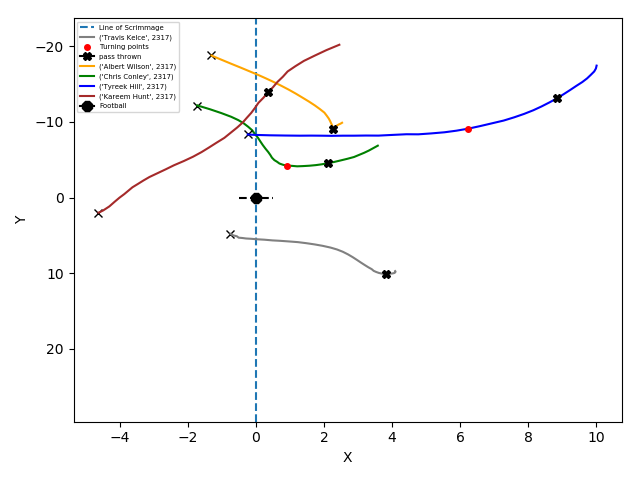
\includegraphics[width=8.89in,angle=360, scale=0.6]{figure/2317} \caption{On the right hand side, Conley and Wilson run a slants, creating traffic. Running back goes to the flat. We can see the brown trajectory of RB intersects with both wide receivers. Play is added to database.}\label{fig:slantflat2}
\end{figure}
\section{Limitations}\label{limitations}

In idenfying slant flat concept, since we are looking for an
intersection close to line of scrimmage, it is possible to get false
flags from certain tight alignments, where receiver trajectories do
intersect in the middle of the field. An example is shown below, where
two tight ends on the right hand side run routes that intersect in the
middle of the field. The observation from six games on the dataset is
that this method can identify three to seven potential plays (out of
\textasciitilde{}75) that have the possibility of including a slant-flat
concept. In our observations, at most three plays are typical slant flat
concepts. We have also observed method also is susceptible to confusing
slant-flant concept with a curl-flat route combination run from certain
alignmnets. Certain important questions remain, as how to generalize a
method that can identify multiple concepts automatically. The final goal
of this project will be to have a fully-automated route concept
identification system based on alignment and route characteristics.

\section{Future Works}\label{future-works}

The first step will be to devise an unsupervised machine learning model
based on k-means to classify routes run by receivers using the widely
accepted route tree. Once we have the model, we can automatically
classify routes and check if certain combinations of routes occur in
certain part of the field. If they do, the methodology that we used
specifically to identfying slant-flat concept can be generalized to
identify other concepts. The end goal should be to extract plays that
run a certain concept from our plays database, so the coaches do not
have to through all of the film tape of NFL matches to see certain
concepts.
\begin{figure}
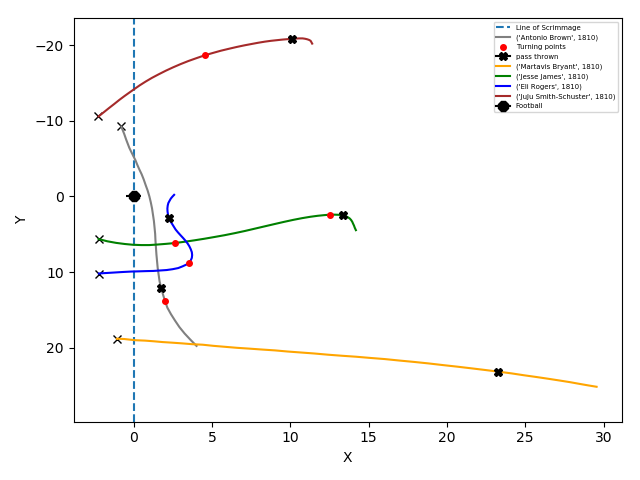
\includegraphics[width=8.89in,angle=360, scale=0.6]{figure/1810} \caption{Blue and green routes run by tight ends intersect within 5 yards. The play is wrongly tagged as slant-flat concept}\label{fig:slantflat3}
\end{figure}
\section{Conclusion}\label{conclusion}

The present work hopes to establish a starting point for the initial
goal of automatically identfying American Football receiver route
concepts. Through a specific example, the slant-flat concept, we explain
the general framework of identfying the route concepts, while touching
on some important route trajectory features that will be important for
the second part of the project, which is to automatically identify
different routes as specified by the route tree using unsupervised
machine learning.

\backmatter

\chapter*{References}\label{references}
\addcontentsline{toc}{chapter}{References}

\markboth{References}{References}

\noindent

\setlength{\parindent}{-0.20in} \setlength{\leftskip}{0.20in}
\setlength{\parskip}{8pt}

\hypertarget{refs}{}
\hypertarget{ref-barnett}{}
Ajmeri, O., \& Sha, A. (2018). Using computer vision and machine
learningto automatically classify nfl game film and develop a player
tracking system. \emph{MIT Sloan Sport Analytics Conference}.

\hypertarget{ref-beckmann}{}
Beckmann, L., \& Budig, B. (2015). There and back again: Using
fréchet-distance diagramsto find trajectory turning points.
\emph{SIGSPATIAL}.

\hypertarget{ref-david}{}
H, D., \& Peucker, T. (1973). Algorithms for the reduction of the number
of points required to represent a digitized line or its caricature.
\emph{Cartographica: The International Journal for Geographic
Information and Geovisualization}.

\hypertarget{ref-jeremy}{}
Jeremy, H., \& Gagnon, P. T. (2017). American football route
identification using supervised machine learning. \emph{MIT Sloan Sport
Analytics Conference}.

\hypertarget{ref-ramer}{}
Urs., R. (1973). An iterative procedure for the polygonal approximation
of plane curves. \emph{Computer Graphics and Image Processing}.


% Index?

\end{document}
